%!TEX root = ../CallenThermo.tex
%翻译:碘化亚铜
%校对:lh, Surgam Identidem
\chapter{其它表象,Legendre变换}
\label{chap5}

\section{能量最小原理}
\label{sec5.1}

之前的章节已经得到了熵最大原理最显著最直接的一些推论,进一步的推论会导出其它很多有用的基本结论。不过本章要重新审视理论的形式框架,并且注意到用一些等价的数学形式可以重新构造出相同的内容,这对深化发展热力学理论十分有益。这些其它的形式(表象)会在一些特殊类型的问题中显得特别方便,而热力学计算的艺术经常体现在选取对于给定的问题最适用的某种形式(表象)上。在恰当的表象下热力学问题会变得极为简单,而在不恰当的表象下会变得极为复杂。

力学中也会出现多种等价的形式——Newton形式,Lagrange形式,Hamilton形式。同样也会有某一问题用Lagrange形式处理会比用Newton形式更加容易处理的请况,反之亦然。但是不同形式(表象)导致的难易不同在热力学中表现得极为显著。正因如此,{\it 等价表象之间的一般变换理论是热统计理论的基础之一}。

之前实际上已经考虑过了两种等价的表象——能量表象和熵表象。但基本的极值原理却只在熵表述中构造出来。如果这两种表述的理论地位相同,我们就必须找出能量表象中与熵最大原理类似的极值原理,它确实存在。熵最大原理等价于能量最小原理,二者可相互替代。熵最大原理表明,在总能量的给定的条件下,平衡态对应于熵取最大值的状态。能量最小原理则表明对于给定总熵的平衡态,能量取最小值。

{
  \centering
  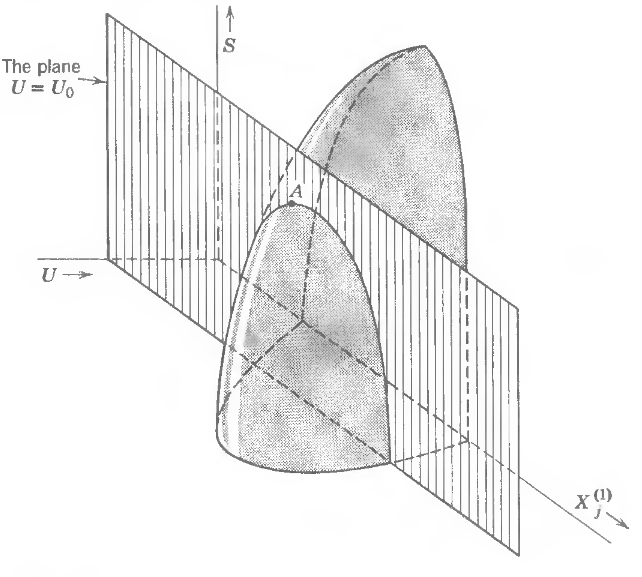
\includegraphics[width=0.6\textwidth]{fig5.1.png}
  \figcaption{平衡态$A$在给定$U$时$S$取极大。}
  \label{fig5.1}
}

图\ref{fig5.1}展示了\ref{sec4.1}节讨论的复合系统位形空间的剖面图。标记为$U$和$S$的轴对应复合系统的总能量和总熵,而标记为$X_j^{(1)}$的轴则对应着第一个子系统的某个广延量。其它没有在图中显示的轴还包括$U^{(1)}$,$X_j$以及其它的$X_k^{(1)}$和$X_k$。

复合系统的总能量是一个由封闭条件决定的常数。这个封闭条件的几何表示是系统的态处于图\ref{fig5.1}中$U=U_0$的平面上。系统的基本方程表示为图中的曲面,因此表示系统状态的点一定位于曲面和平面相交得到的曲线上。如果参数$X_j^{(1)}$不受约束,那么平衡态就是曲线上使得熵最大的态,也就是图\ref{fig5.1}中标记为A的态。

{
	\centering
	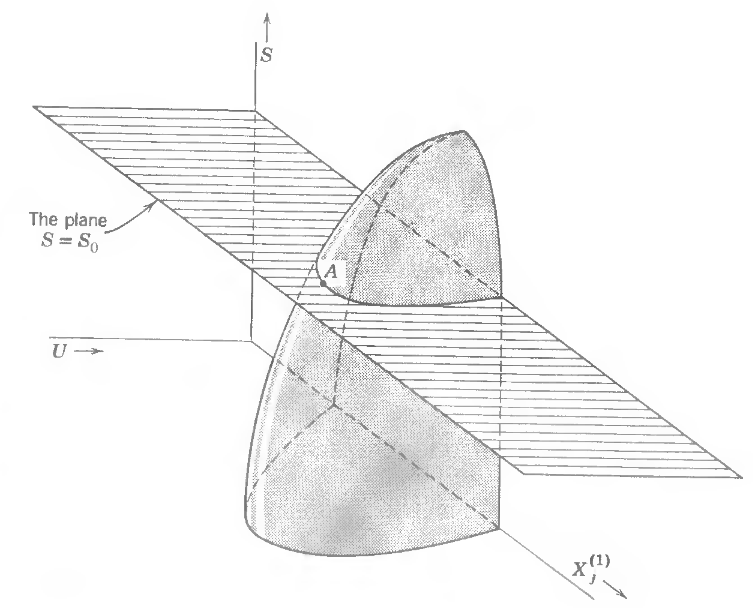
\includegraphics[width=0.6\textwidth]{fig5.2.png}
	\figcaption{平衡态$A$在给定$S$时$U$取极小。}
	\label{fig5.2}
}

在另一种表象下,平衡态A可以视为给定熵的能量最小态 —— 如图\ref{fig5.2}所示。经过平衡态点A的平面$S=S_0$与基本曲面\mpar{基本方程所对应的曲面}相交定义了一条曲线。这条曲线包含了一族熵为常数的态,{\it 而平衡态A则是曲线上能量最小的态}。

如图\ref{fig5.1}和\ref{fig5.2}所示,熵最大和能量最小原理的等价性明确依赖于基本曲面的几何形状,这个性质是普遍的。\ref{sec4.1}节讨论过,基本曲面的形状是由$\partial S/\partial U>0$以及$U$是关于$S$的单值连续函数这两个假设决定的;因此这两个关于解析性质的假设是两个原理等价的隐含条件。

总结一下,尽管尚未证明,但以下两个原理看起来是等价的:

{\bf 熵最大原理.}{\it 在总的内部能量确定时,任何不受约束的内部参量在平衡时的取值都使得熵最大}。

{\bf 能量最小原理.}{\it 在总的熵确定时,任何不受约束的内部参量在平衡时的取值都使得能量最小}。

两个极值准则等价性的证明既可以用物理论证,也可以用数学的方式阐述。首先考虑物理论证,下面说明如果能量{\it 不是}最小值的话,熵就可以不是最大值,并且反之亦然。

假设系统处于平衡态但能量并{\it 不是}在给定的熵下可能的最小值。这样就可以在保持熵为常数的同时从系统中提取能量(通过做功),并且随后就可以通过传热把这部分能量返还给系统。这样系统的熵会增加($\dbar Q=T\, \rd S$),于是系统恢复到它初始的能量,但是熵增加了。这跟初始的平衡态是熵最大的态是矛盾的!因此我们不得不推断最初的平衡态必须具有给定的熵下最小的能量。

相反的推论,也就是最小能量要求最大的熵,可以用类似的方式构造(见习题5.1-1).

下面是更形式化的证明,先假设熵最大原理成立:
\begin{equation}
\label{equ5.1}
\left(\frac{\partial S}{\partial X}\right)_U=0
~\text{及}~
\left(\frac{\partial^2 S}{\partial X^2}\right)_U<0
\end{equation}
在此为了简便,我们将$X_j^{(1)}$写作$X_j$,这暗示着其它的$X$将保持为常数。同时为了简便,我们暂时将一阶导数$(\partial U/\partial X)_S$记为$P$。于是根据(根据附录A中的公式A.22)可得:
\begin{equation}
\label{equ5.2}
	P \equiv \left( \frac{\partial U}{\partial X} \right)_S = -\frac{ \left( \dfrac{\partial S}{\partial X} \right)_U }{ \left( \dfrac{\partial S}{\partial U}\right)_X } = -T \left(\frac{\partial S}{\partial X}\right)_U = 0
\end{equation}
由此可推断$U$是极值。为了分清这个极值是极大极小还是拐点,我们必须研究二阶导数$(\partial^2U/\partial X^2)_S\equiv(\partial P/\partial X)_S$的正负。但是如果将$P$当做$U$和$X$的函数,则有:
\begin{align}
	\left(\frac{\partial^2 U}{\partial X^2}\right)_S &=\left(\frac{\partial P}{\partial X}\right)_S =\left(\frac{\partial P}{\partial U}\right)_X \left(\frac{\partial U}{\partial X}\right)_S +\left(\frac{\partial P}{\partial X}\right)_U =\left(\frac{\partial P}{\partial U}\right)_XP +\left(\frac{\partial P}{\partial X}\right)_U \label{equ5.3} \\
	&= \left( \frac{\partial P}{\partial X} \right)_U. \quad (P=0) \label{equ5.4} \\
	&= \frac{\partial}{\partial X} \left[- \frac{ \left( \dfrac{\partial S}{\partial X} \right)_U }{ \left( \dfrac{\partial S}{\partial U}\right)_X } \right]_U \label{equ5.5} \\
	&= -\frac{\dfrac{\partial^2 S}{\partial X^2}} {\dfrac{\partial S}{\partial U}} + \frac{\partial S}{\partial X} \frac{\dfrac{\partial^2 S}{\partial X \partial U}}{\left(\dfrac{\partial S}{\partial U}\right)^2} \label{equ5.6} \\
	&= -T\frac{\partial^2 S}{\partial X^2}>0 \quad \left( \frac{\partial S}{\partial X}=0 \right) \label{equ5.7}
\end{align}
因此$U$是一个极小值。反向的论证在形式上是一样的。

以前说过,两个极值条件完全等价的事实类似于几何中的等周问题。也就是一个圆既可以描述为给定周长下面积最大的二维图形,也可以描述为给定面积下周长最小的二维图形。

这两个描述圆的极值条件是完全等价的,每一个都适用于所有的圆。只不过它们给出两种不同的生成圆的方法。如果要把正方形连续变形为一个圆,我们可以保持它的面积是常数并且允许它的边像橡皮筋一样收缩。这样我们得到了作为给定面积下周长最小图形的一个圆。等价地,我们也可以保持正方形的周长不变并允许面积增加,这样就得到了作为给定周长下面积最大图形的一个(不同的)圆。尽管如此,在得到这些圆之后,{\it 每一个圆都同时满足自身取值下面积和周长的极值条件}。

关于热力学系统的物理情形跟上面描述的几何情形是非常类似的。也就是说,任何一个平衡态既可以描述为给定能量下熵最大的态,也可以描述为给定熵下能量最小的态。但是这两个条件却给出了两个不同的达到平衡态的方法。

作为这两种达到平衡方法的一个特定的例子,考虑一个最初固定在封闭圆柱某个位置的活塞。如何在移除活塞位置的限制之后使系统达到平衡态?我们可以简单地移去约束来使它自发达到平衡;此时由于封闭条件,能量会保持为常数而熵会增加。这个过程就是熵最大原理所要求的过程。此外,我们可以让活塞非常缓慢地移动,可逆地对外做功直到它到达两边压强相等的位置。在这个过程中能量从系统中提取出来,但是系统的熵保持为常数(这个过程是可逆的且没有热流)。这个过程就是能量最小原理要求的过程。
我们想强调的关键事实是,{\it 这两个过程以及其它任意过程最终达到的平衡态都满足两大极值原理。}%
\mpar{当然,从一个初态出发,通过不同的过程会到达不同的平衡态。}%
。

为了进一步说明最小能量原理,下面用它来解决\ref{sec2.4}节的热平衡问题(那里是用最大熵原理解决的)。考虑内部由固定的透热壁分隔的封闭复合系统,热量可以在两个子系统间自由流动,下面来找出它的平衡态。

能量表象下的基本方程是
\begin{equation}
\label{equ5.8}
U=U^{(1)}(S^{(1)},V^{(1)},N^{(1)}_1,\ldots)+U^{(2)}(S^{(2)},V^{(2)},N^{(2)}_1,\ldots)
\end{equation}
所有的体积和摩尔数都是已知常数,需要计算$S^{(1)}$和$S^{(2)}$。
暂时忽略系统封闭导致的总能量不变的事实,{\it 如果}允许能量改变的话,平衡态对应于能量最小的态。两个子系统之间虚拟热流引起总能量的虚拟变化为:
\begin{equation}
\label{equ5.9}
\,\mathrm dU=T^{(1)}\,\mathrm dS^{(1)}+T^{(2)}\,\mathrm dS^{(2)}
\end{equation}
能量最小条件也就是$\rd U = 0$,在总熵不变的条件下:
\begin{equation}
\label{equ5.10}
S^{(1)}+S^{(2)}=\text{constant}
\end{equation}
会有
\begin{equation}
\label{equ5.11}
\mathrm dU=(T^{(1)}-T^{(2)})\,\mathrm dS^{(1)}=0
\end{equation}
于是可得
\begin{equation}
\label{equ5.12}
T^{(1)}=T^{(2)}
\end{equation}

从而能量最小原理给出了与前面用熵最大原理得到的相同的热平衡条件。

方程\eqref{equ5.12}是一个关于$S^{(1)}$和$S^{(2)}$的方程。在总能量$U$已知,因此仅有的两个未知量是$S^{(1)}$和$S^{(2)}$的情况下,第二个方程选为方程\eqref{equ5.8}最为方便。理论上方程\eqref{equ5.8}和\eqref{equ5.12}会给出这个问题的精确解。

用完全一样的思路,可以发现一个内部有可动绝热壁的封闭系统的平衡条件是压强相等。这个结论在能量表象中是非常直接的,但是如同在\ref{sec2.7}的最后一段看到的,在熵表象中相对更加微妙。

\subsection*{习题}

\section{Legendre变换}
\label{sec5.2}

在能量表象和熵表象中,广延量都作为数学上的独立变量,而强度量都视为被导出的物理量。这与现实中实验操作的便利性截然不同。实验者经常发现强度量更容易测量和控制,因此更喜欢把强度量当成操作上的独立变量而把广延量当成导出量。最突出的是熵和温度这一对共轭变量:并不存在可以测量和控制熵的实验仪器,而测量和控制温度的温度计和恒温器在实验室中十分常见。于是,能否改变数学形式使得强度量代替广延量成为数学上的独立变量?当然可以,而且这样还能够导出很多其它的热力学表象。

重要的事情说三遍:不论是在熵表象还是能量表象下热力学都是逻辑完备且独立的,而介绍这些表象变换只是为了方便。大家公认这是一种使热力学避免了繁琐推导的简化。但原则上讲这只是某种捷径,并不是逻辑上所必须的。

下面给出表象变换的严格表述。设系统的基本方程已知:
\begin{equation}
\label{equ5.13}
	Y=Y(X_0,X_1,\ldots,X_l)
\end{equation}
我们想找到一个将导数
\begin{equation}
\label{equ5.14}
	P_k\equiv\frac{\partial Y}{\partial X_k}
\end{equation}
作为独立变量,但是不改变基本关系\eqref{equ5.13}中任何其他信息的方法。在几何和其他一些物理领域中也有与之类似的问题。这个问题需要采用名为Legendre变换的数学手段,它的几何意义十分直观,下面先来介绍Legendre变换的几何意义。

{
	\centering
	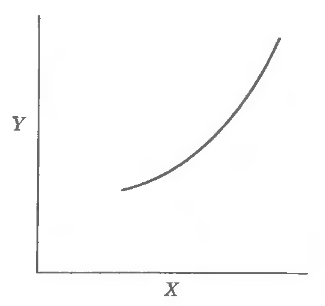
\includegraphics[width=.5\textwidth]{fig5.3.png}
	\figcaption{}
	\label{fig5.3}
}

简便起见,首先考虑基本方程只与一个独立变量$X$有关的情形:
\begin{equation}
\label{equ5.15}
	Y=Y(X)
\end{equation}
几何上,这个基本关系可表为直角坐标$X, Y$空间中的一条曲线(图\ref{fig5.3}),而导数
\begin{equation}
\label{equ5.16}
	P\equiv\frac{\partial Y}{\partial X}
\end{equation}
是这个曲线的切线斜率。如果想用$P$代替$X$作为独立变量,我们的第一反应可能是简单地用方程\eqref{equ5.15}和\eqref{equ5.16}消去$X$,从而得到$Y$关于$P$的函数
\begin{equation}
\label{equ5.17}
	Y=Y(P)
\end{equation}
从几何上容易看出,这样做无论如何都会在数学上牺牲掉基本关系\eqref{equ5.15}式的一些信息。显然对于$Y$关于斜率$dY/dX$的函数的了解并不能让我们重构出曲线$Y=Y(X)$。实际上,图\ref{fig5.4}中每一条替代的曲线都等价地满足关系$Y=Y(P)$。
从分析的观点来看,关系$Y=Y(P)$是一个一阶微分方程,而它的积分给出的结果跟$Y=Y(X)$差一个待定的积分常数。由此可见,如果用$Y=Y(P)$代替$Y=Y(X)$成为基本方程,就会丢失掉基本关系中的一些原始信息。尽管我们希望让$P$成为一个数学上的独立变量,但这样做导致的信息丢失使得该方案完全不可行。

{
	\centering
	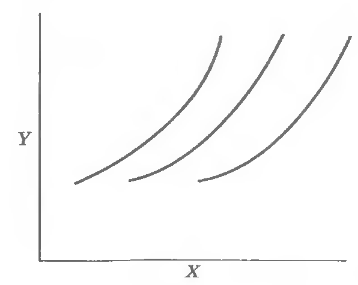
\includegraphics[width=0.6\textwidth]{Pictures/fig5.4.png}
	\figcaption{}
	\label{fig5.4}
}

靠谱的做法是由传统的{\it 点几何(point geometry)}与Pluecker的{\it 线几何(line geometry)}的对偶关系给出的。线几何的基本概念是一条给定的曲线可以很好地由以下两种方式等价描述:

\begin{itemize}
\item[(a)] 作为一族切线的包络线(图\ref{fig5.5});
\item[(b)] 作为满足关系$Y=Y(X)$的点的轨迹。
\end{itemize}

任何可以构造出一族切线的方程都能和关系$Y=Y(X)$一样好地决定一条曲线。

{
	\centering
	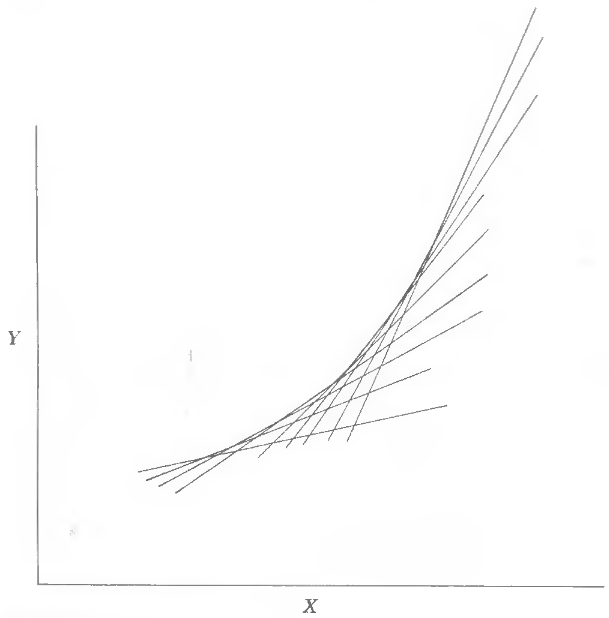
\includegraphics[width=0.5\textwidth]{Pictures/fig5.5.png}
	\figcaption{}
	\label{fig5.5}
}

正如平面上的每一个点都可以由两个数$X$和$Y$描述,平面上的每一条直线也都可以用两个数$P$和$\psi$描述,其中$P$是直线的斜率,$\psi$是它在$Y$轴上的截距。于是正如关系$Y=Y(X)$挑出了所有可能的点$(X,Y)$中的一个子集,关系$\psi=\psi(P)$挑出了所有可能的直线$(P,\psi)$的一个子集。关于切线的截距$\psi$作为斜率$P$的函数的知识可以让我们构造出一族切线,从而也就构造出了它们的包络线,也就是这条曲线。因此关系
\begin{equation}
\label{equ5.18}
	\psi=\psi(P)
\end{equation}
是跟基本关系$Y=Y(X)$完全等价的。在这个关系中,独立变量是$P$,于是方程\eqref{equ5.18}给出了对于自变量替换问题的一个圆满的解。由于关系$\psi=\psi(P)$跟关系$Y=Y(X)$是数学等价的,所以它也可以当成一个基本关系;$Y=Y(X)$是“$Y$表象”下的基本关系,而$\psi=\psi(P)$是“$\psi$表象”下的基本关系。

建议读者去画一些不同的斜率$P$和不同的$Y$轴截距$\psi=-P^2$的直线。可以看出关系$\psi=-P^2$描述了一条抛物线(常用的描述是$Y=\frac{1}{4}X^2$)。在“$\psi$表象”下抛物线的基本方程是$\psi=-P^2$,而“$Y$表象”下同一条抛物线的基本方程是$Y=\frac{1}{4}X^2$。

{
	\centering
	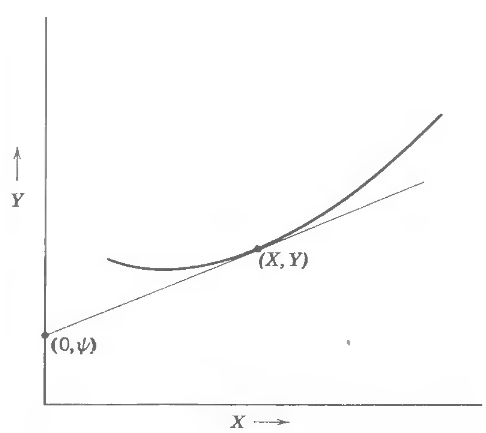
\includegraphics[width=.7\textwidth]{fig5.6.png}
	\figcaption{}
	\label{fig5.6}
}

现在的问题是给出关系$Y=Y(X)$后如何计算$\psi=\psi(P)$。相应的数学操作称为Legendre变换。考虑一条经过点$(X,Y)$,斜率为$P$的切线。如果截距是$\psi$,则有(见图\ref{fig5.6})
\begin{equation}
\label{equ5.19}
	P=\frac{Y-\psi}{X-0}
\end{equation}
或者
\begin{equation}
\label{equ5.20}
	\psi=Y-PX
\end{equation}

基本方程已经给出:
\begin{equation}
\label{equ5.21}
	Y=Y(X)
\end{equation}
并且通过求导可以得到
\begin{equation}
\label{equ5.22}
	P=P(X)
\end{equation}
于是联立方程\eqref{equ5.20}、\eqref{equ5.21}和\eqref{equ5.22}消去%
\footnote{只有在$P$与$X$有关(也就是$\rd^2 Y / \rd X^2 \neq 0$)的情况下才能消去$X, Y$,这在热力学对应于稳定性的要求。这个条件只有在“临界点”才会失效,相关内容在第\ref{chap10}章讨论。}%
$X$和$Y$我们就能得到想要的$\psi$和$P$之间的关系。Legendre变换的基本等式就是方程\eqref{equ5.20},而这个方程可以当成函数$\psi$的解析定义。函数$\psi$称为$Y$的{\it Legendre变换(Legendre transformation)}。

相反的问题是给出关系$\psi=\psi(P)$,重新求出关系$Y=Y(X)$。可以看出$(X,Y)$和$(\psi,P)$之间的关系跟它的逆关系是对称的,区别只是Legendre的方程中差了一个负号。
对方程\eqref{equ5.20}求导并且应用$\,\mathrm dY=P\,\mathrm dX$可得
\begin{align}
\label{equ5.23}
	\,\mathrm d\psi &= \,\mathrm dY-P\,\mathrm dX-X\,\mathrm dP \nonumber \\
	~ &= -X\,\mathrm dP
\end{align}
也就是
\begin{equation}
\label{equ5.24}
	-X=\frac{\mathrm d\psi}{\mathrm dP}
\end{equation}
如果从给出的方程$\psi=\psi(P)$和方程\eqref{equ5.24}和\eqref{equ5.20}中消去%
\footnote{这样做可能的条件是$\rd^2\psi/\rd P^2\neq0$,在热力学中是由所考虑系统的稳定性保证的。}%
两个变量$\psi$和$P$,我们就重构出了关系$Y=Y(X)$。Legendre变换与其逆的对称性可以通过下表对比看出:

{{\centering
\begin{equation*}
\begin{array}{c|c}
\hline
Y=Y(X) & \psi=\psi(P) \\
P=\dfrac{\mathrm dY}{\mathrm dX} & -X=\dfrac{\mathrm d\psi}{\mathrm dP} \\
\psi=-PX+Y & Y=XP+\psi \\
\text{消掉$X$和$Y$得到} & \text{消掉$P$和$\psi$得到} \\
\psi=\psi(P) & Y=Y(X)\\
\hline
\end{array}
\end{equation*}
}}

容易将Legendre变换推广到不止一个独立变量的函数。在三维中,$Y$是关于$X_0$和$X_1$的函数,基本方程表示一个曲面。这个曲面可以当成满足基本方程$Y=Y(X_0,X_1)$的点的轨迹,或者当成切平面的包络面。一个平面可以用在在$Y$轴上的截距$\psi$和在$Y-X_0$以及$Y-X_1$平面上的截线的斜率$P_0$和$P_1$来刻画。于是基本方程就是所有可能的平面中用$\psi=\psi(P_0,P_1)$描述的子集。

基本方程的一般形式
\begin{equation}
\label{equ5.25}
	Y=Y(X_0,X_1,\dots,X_t)
\end{equation}
表示了一个在直角坐标$Y,X_0,X_1,\dots,X_t$的$(t+2)$维空间中的超平面。导数
\begin{equation}
\label{equ5.26}
	P_k=\frac{\partial Y}{\partial X_k}
\end{equation}
是曲面的偏斜率。超曲面可以等价地用满足方程\eqref{equ5.25}描述的点的轨迹或者切超平面的包络来描述。切超平面族可以用超平面的截距$\psi$关于斜率$P_0,P_1,\dots,P_t$的函数来刻画。
于是
\begin{equation}
\label{equ5.27}
	\psi=Y-\sum_kP_kX_k
\end{equation}
对上式微分可得
\begin{equation}
\label{equ5.28}
	\,\mathrm d\psi=-\sum_kX_k\,\mathrm dP_k
\end{equation}
从而
\begin{equation}
\label{equ5.29}
	-X_k = \frac{\partial \psi}{\partial P_k}
\end{equation}
Legendre变换实现了从$Y=Y(X_0,X_1,\dots,X_t)$、方程组\eqref{equ5.26}和方程\eqref{equ5.27}中消去$Y$和$X_k$。逆变换实现了从$\psi=\psi(P_0,P_1,\dots,P_r)$、方程组\eqref{equ5.29}和方程\eqref{equ5.27}中消去$Y$和$X_k$。

最后,Legendre变换可以仅仅在关系$Y=Y(X_0,X_1,\dots,X_t)$的$(t+2)$维全空间中的一个$(n+2)$维子空间中进行。显然这个子空间必须包含$Y$坐标,但是可以包含集合$X_0,X_1,\dots,X_t$中的任选$n+1$个坐标。为了记号上的方便,我们排列坐标使得Legendre变换作用在前$n+1$个坐标(以及$Y$)构成的子空间上;坐标$X_{n+1},X_{n+2},\dots,X_t$保持不变。这样一个部分Legendre变换的作用只不过是在变换中把$X_{n+1},X_{n+2},\dots,X_t$当成常数。这样的Legendre变换必须用符号标出哪些独立变量参与了变换。我们引入标记$Y[P_0,P_1,\dots,P_n]$来标记对函数$Y(X_0,X_1,\dots,X_t)$做对应于$X_0,X_1,\dots,X_n$的Legendre变换。从而$Y[P_0,P_1,\dots,P_n]$就是一个关于独立变量$P_0,P_1,\dots,P_n,X_{n+1},\dots,X_t$的函数。
在接下来的表中展示了在部分Legendre变换和它的逆变换中包含的各种关系。

\begin{tabularx}{1.4\textwidth}{X|X}
\hline
  $Y=Y(X_0,X_1,\dots,X_t)$ & \begin{mymath}Y[P_0, P_1, \dots, P_n] = P_0, P_1, \dots, P_n, X_{n+1}, \dots, X_t \, \text{的函数}\label{equ5.30}\end{mymath}\\
  $P_k = \frac{\partial Y}{\partial X_k}$ & \begin{mymath}-X_k = \frac{\partial Y[P_0,\dots,P_n]}{\partial P_k}, \quad k\leq n\label{equ5.31}\end{mymath} \\
   & $P_k = \frac{\partial Y[P_0,\dots,P_n]}{\partial X_k}\quad k > n$ \\
  偏微分表示了$Y$的所有除了$X_k$以外的自然变量(比如所有满足$j\neq k$的$X_j$) & 偏微分表示了$Y[P_0,\dots,P_n]$除了已经包含了其偏微分以外的所有自然变量。 \\
  $\,\mathrm dY=\sum_0^t P_k\,\mathrm dX_k$ & \begin{mymath}\mathrm dY[P_0, \dots, P_n] = -\sum_0^n X_k \,\mathrm dP_k + \sum_{n + 1}^t P_k \,\mathrm dX_k \label{equ5.32}\end{mymath}\\
  $Y[P_0,\dots,P_n]=Y-\sum_0^nP_kX_k$ & \begin{mymath}Y=Y[P_0,\dots,P_n]+\sum_0^nX_kP_k\label{equ5.33}\end{mymath} \\
  从方程(5.30),(5.33)和(5.31)的前$n+1$个方程中消除掉$Y$和$X_0, X_1,\dots,X_n$可以导出变换后的基本关系。 & 从方程(5.30),(5.33)和(5.31)的前$n+1$个方程中消除掉$Y[P_0, \dots, P_n]$和$P_0, P_1, \dots, P_n$可以导出原始的基本关系。\\
  \hline
\end{tabularx}

本节讲述了Legendre变换的数学形式,而未涉及其物理应用。在介绍热力学的应用之前,我们指出它在物理学中相比热力学更为人熟知的一个领域——Lagrangian和Hamiltonian力学中的应用。Lagrange原理宣称,存在一个特殊的函数Lagrangian\mpar{通译为“拉格朗日量”或简称“拉氏量”,本书英文人名一律不译。},完整刻画了一个力学系统的动力学。Lagrangian是一个关于$2r$个变量的函数,其中$r$个是{\it 广义坐标(generalized coordinates)},$r$个是{\it 广义速度(generalized velocities)}。因此方程
\begin{equation}
\label{equ5.34}
	L=L(v_1,v_2,\dots,v_r,q_1,q_2,\dots,q_r)
\end{equation}
扮演了基本关系的角色。

{\it 广义动量(generalized momenta)}定义成Lagrangian的导数
\begin{equation}
\label{equ5.35}
	P_k \equiv \frac{\partial L}{\partial v_k}
\end{equation}
如果想要用动量代替速度作为独立变量,我们必须做关于速度的部分Legendre变换。
从而我们引入一个新的函数,叫做Hamiltonian\mpar{通译为“哈密顿量” \sout{越来越多的人采用“蛤密顿量”以纪念长者},本书英文人名一律不译。},定义是%
\footnote{我们约定Lagrangian的Legendre变换是{\it 负}的Hamiltonian。实际上,数学上的约定和力学中的是一样的,而函数$-\psi$会被叫做$Y$的Legendre变换}%
\begin{equation}
\label{equ5.36}
	(-H)=L-\sum_{k = 1}^r P_kv_k
\end{equation}
然后一个完整的动力学形式就可以基于这个新的基本关系给出
\begin{equation}
\label{equ5.37}
  H=H(P_1,P_2,\dots,P_r,q_1,q_2,\dots,q_r)
\end{equation}
此外,根据方程(5.31), $H$的关于$P_k$的导数是速度$v_k$,也就是Hamilton动力学方程之一。因此如果形如\eqref{equ5.34}式的一个方程被当成Lagrangian力学的动力学方程,那么Hamilton方程\eqref{equ5.37}就是Hamiltonian力学中等价的基本方程。

\subsection*{习题}

\section{热力学势}
\label{sec5.3}
前面介绍的形式在热力学中的应用是不言自明的。基本关系$Y=Y(X_0,X_1,\dots)$可以解释为能量表象的基本关系$U=U(S,X_1,X_2,\dots,X_t)$或者$U=U(S,V,N_1,N_2,\dots)$。而偏导数$P_0,P_1,\dots$对应着强度量$T,-P,\mu_1,\mu_2,\dots$。
Legendre变换后的函数叫做{\it 热力学势},而现在我们明确定义它们中最常见的几个。在第\ref{chap6}章中将通过每一个势的极值原理继续关于这些函数的讨论,表明每一个的直观意义,并且讨论在热力学理论中它们的特殊角色。但下面只关注几个特定的函数的形式化定义。

{\it Helmholtz势(Helmholtz potential)}或者{\it Helmholtz自由能(Helmholtz free energy)},是$U$用温度代替熵成为独立变量的Legendre变换得到的。按国际标准,Helmholtz势的符号是$F$。Helmholtz势的自然变量是$T,V,N_1,N_2,\dots$。
也就是函数关系$F=F(T,V,N_1,N_2,\dots)$构成一个基本关系。按\ref{sec5.2}节规定的记号:
\begin{equation}
\label{equ5.38}
	F\equiv U[T]
\end{equation}

能量表象和Helmholtz表象的完整关系总结在了下面的对比表中:

\begin{tabular}{c|c}
\hline
$U=U(S,V,N_1,N_2,\dots)$ & \begin{mymath}F=F(T,V,N_1,N_2,\dots)\label{equ5.39}\end{mymath}\\
$T=\partial U/\partial S$ & \begin{mymath}-S=\partial F/\partial T\label{equ5.40} \end{mymath}\\
$F=U-TS$ & \begin{mymath}U=F+TS \label{equ5.41} \end{mymath}\\
消去$U$和$S$得到 & 消去$F$和$T$得到\\
$F=F(T,V,N_1,N_2,\dots)$ & $U=U(S,V,N_1,N_2,\dots)$\\
\hline
\end{tabular}

全微分$\mathrm dF$是
\begin{equation}
\label{equ5.42}
  \,\mathrm dF=-S\,\mathrm dT-P\,\mathrm dV+\mu_1\,\mathrm dN_1+\mu_2\,\mathrm dN_2+\cdots
\end{equation}

{\it 焓(enthalpy)}是$U$用压强代替体积成为独立变量的Legendre变换得到的。按照国际物理学会和化学学会的建议,以及与基本\sout{用}法保持一致,我们用符号$H$来标记焓。这个势的自然变量是$S,P,N_1,N_2,\dots$,
\begin{equation}
\label{equ5.43}
	H\equiv U[P]
\end{equation}
能量表象和焓表象的关系表如下:

\begin{tabular}{c|c}
\hline
$U=U(S,V,N_1,N_2,\dots)$ & \begin{mymath}H=H(S,P,N_1,N_2,\dots)\label{equ5.44}\end{mymath}\\
$-P=\partial U/\partial V$ & \begin{mymath}V=\partial H/\partial P\label{equ5.45} \end{mymath}\\
$H=U+PV$ & \begin{mymath}U=H-PV \label{equ5.46} \end{mymath}\\
\text{消去$U$和$V$得到} & \text{消去$H$和$P$得到}\\
$H=H(S,P,N_1,N_2,\dots)$ & $U=U(S,V,N_1,N_2,\dots)$\\
\hline
\end{tabular}

需要特别注意的是方程(5.45)和(5.46)的正负不同,这是由于$-P$是对应于$V$的强度量。

全微分$\mathrm dH$是
\begin{equation}
\label{equ5.47}
	\mathrm dH=T\,\mathrm dS+V\,\mathrm dP+\mu_1\,\mathrm dN_1+\mu_2\,\mathrm dN_2+\dots
\end{equation}

第三个常用的能量的Legendre变换是{\it Gibbs势(Gibbs potential)},或者叫{\it Gibbs自由能(Gibbs free energy)}。这个势是同时用温度代替熵并用压强代替体积作为独立变量的Legendre变换。标准的记号是$G$,而自然变量是$T,P,N_1,N_2,\dots$。
从而有
\begin{equation}
\label{equ5.48}
  G\equiv U[T,P]
\end{equation}
以及

\begin{tabular}{c|c}
\hline
$U=U(S,V,N_1,N_2,\dots)$ & \begin{mymath}G=G(T,P,N_1,N_2,\dots)\label{equ5.49}\end{mymath}\\
$T=\partial U/\partial S$ & \begin{mymath}-S=\partial G/\partial T\label{equ5.50} \end{mymath}\\
$-P=\partial U/\partial V$ & \begin{mymath}V=\partial G/\partial P\label{equ5.51} \end{mymath}\\
$G=U-TS+PV$ & \begin{mymath}U=G+TS-PV \label{equ5.52} \end{mymath}\\
消去$U$,$S$和$V$得到 & 消去$G$,$T$和$P$得到\\
$G=G(T,P,N_1,N_2,\dots)$ & $U=U(S,V,N_1,N_2,\dots)$\\
\hline
\end{tabular}

全微分$\mathrm dG$是
\begin{equation}
\label{equ5.53}
	\,\mathrm dG=-S\,\mathrm dT+V\,\mathrm dP+\mu_1\,\mathrm dN_1+\mu_2\,\mathrm dN_2+\dots
\end{equation}

{\it 巨正则势}$U[T,\mu]$是在统计力学中自然出现的热力学势,对于这个势有:

\begin{tabular}{c|c}
\hline
$U=U(S,V,N)$ & \begin{mymath}U[T,\mu]=T,V,\text{和}\mu\text{的函数}\label{equ5.54}\end{mymath}\\
$T=\partial U/\partial S$ & \begin{mymath}-S=\partial U[T,\mu]/\partial T\label{equ5.55} \end{mymath}\\
$\mu=\partial U/\partial N$ & \begin{mymath}-N=\partial U[T,\mu]/\partial\mu\label{equ5.56} \end{mymath}\\
$U[T,\mu]=U-TS-\mu N$ & \begin{mymath}U=U[T,\mu]+TS+\mu N \label{equ5.57} \end{mymath}\\
消去$U$,$S$和$N$得到 & 消去$U[T,\mu]$,$T$和$P$得到\\
$T,V,\mu$的函数$U[T,\mu]$ & $U=U(S,V,N)$\\
\hline
\end{tabular}

以及
\begin{equation}
\mathrm dU[T,\mu] = -S\,\mathrm dT -P\,\mathrm dV-N\,\mathrm d\mu
\label{equ5.58}
\end{equation}

简单系统内能$U$的其他可能的Legenre变换,如$U[\mu_1]$,$U[P,\mu_1]$,$U[T,\mu_1,\mu_2]$等等,由于不常用而没有通用的命名。完全的Legendre变换是$U[T,P,\mu_1,\mu_2,\dots,\mu_r]$,$U(S,V,N_1,N_2,\dots,N_t)$是它自变量的一阶齐次函数,这导致了$U[T,P,\mu_1,\mu_2,\dots,\mu_r]$恒等于0:

对于
\begin{equation}
\label{equ5.59}
	U[T,P,\mu_1,\mu_2,\dots,\mu_r]=U-TS+PV-\mu_1N_1-\mu_2N_2-\cdots-\mu_rN_r
\end{equation}
根据Euler关系\eqref{equ3.6}式,上式恒等于零:
\begin{equation}
\label{equ5.60}
	U[T,P,\mu_1,\mu_2,\dots,\mu_r]\equiv 0
\end{equation}

\subsection*{习题}

\section{推广的Massieu函数}
\label{sec5.4}
Legendre变换定义的最常用的函数就是\ref{sec5.3}节中提到的那些,此外可以对熵而不是能量做Legendre变换。也就是形如$S=S(U,V,N_1,N_2,\dots)$的基本关系可以当成变换作用的关系。这种对熵的Legendre变换是1869年Massieu发明的,并且提前得到了Gibbs在1875年引入的对能量的变换。
我们把对于熵的变换叫做{\it Massieu函数(Massieu functions)},用来跟从能量变换得到的{\it 热力学势(thermodynamics potentials)}做出区分。
Massieu函数在不可逆热力学的理论中会特别有用,并且在统计力学以及热涨落理论中会自然出现。
三个典型的Massieu函数包括$S[1/T]$,其中温度的倒数代替能量成为了独立变量;$S[P/T]$,其中$P/T$代替体积成为了独立变量;以及$S[1/T,P/T]$,两个替换同时进行。显然
\begin{equation}
\label{equ5.61}\
  S\left[\frac{1}{T}\right]\equiv S-\frac{1}{T}U=-\frac{F}{T}
\end{equation}
\begin{equation}
\label{equ5.62}\
  S\left[\frac{P}{T}\right]\equiv S-\frac{P}{T}\cdot V
\end{equation}
以及
\begin{equation}
\label{equ5.63}\
  S\left[\frac{1}{T},\frac{P}{T}\right]\equiv S-\frac{1}{T}U-\frac{P}{T}\cdot V=-\frac{G}{T}
\end{equation}
从而,这三个中只有$S[P/T]$是不平凡地依赖于前面介绍过的某一个热力学势的。
对于这个函数有:

\begin{tabular}{c|c}
\hline
$S=S(U,V,N_1,N_2,\dots) $& \begin{mymath}S[P/T]=U,P/T,N_1,N_2\text{的函数}\label{equ5.64}\end{mymath}\\
$P/T=\partial S/\partial V $& \begin{mymath}-V=\partial S[P/T]/\partial(P/T)\label{equ5.65} \end{mymath}\\
$S[P/T]=S-(P/T)V $& \begin{mymath}S=S[P/T]+(P/T)V \label{equ5.66} \end{mymath}\\
消去$S$和$V$得到 & 消去$S[P/T]$和$P/T$得到\\
$U,P/T,N_1,N_2,\dots$的函数$S[P/T]$ & $S=S(U,V,N_1,N_2,\dots)$ \\
\hline
\end{tabular}

以及
\begin{equation}
\label{equ5.67}
	\rd S[P/T]=(1/T) \rd U-V \rd (P/T)-(\mu_1/T) \rd N_1-(\mu_2/T) \rd N_2\dots
\end{equation}
其它的Massieu函数可以在读者在特殊情况下用到它们时自己定义和分析。

\subsection*{习题}
